
%!TEX ROOT=slehokri_bp.tex


\chapter{Hardware}
\label{chap:hw}
\section{Indroduction}
\label{sec:hw_intro}


\section{Chassis and transmitter}
\label{sec:hw_base}
\subsection{Background}
The whole project is built on an old entry-level onroad 1/10 chassis from the Tamiya Quick Drive series released on Jul 16, 2003 [TODO: citace]. The RC car was obtained as a childhood gift. It was pre-assembled and came with a 2-channel transmitter communicating at a frequency of 27MHz. Later the servo broke, and no repair or upgrade parts were available. Since the repair was nearly impossible, but the rest of the chassis was fully functional, it was the perfect choice for a complete rebuild.

The car featured a sealed gearbox, servo, "280" size brushed motor and 9.6V Ni-Cd battery pack. Due to the age of the product, not much technical information can be found. %TODO siunitx

\subsection{Modifications}
All the electronics were removed, leaving only the plastic chassis. The broken 5-wire servo was replaced with a "standard" size hobby servo used in most 1/10 RC cars [TODO: info]. The old brushed motor was still functional, but it was decided to replace it with a newer and more powerful one. The only constraint was a shaft size, as the old pinion had to be transferred to the new motor to maintain functionality. Therefore a GoolRC 2435 4800KV BLDC motor with a 25A ESC was chosen.  Table \ref{tab:BLDC_spec} shows motor specifications, and table \ref{tab:ESC_spec} ESC specifications. Furthermore, the plastic bearings were replaced by metal ball bearings. %TODO siunitx

A 2-cell LiPo battery with a capacity of 2200mAh was chosen to supply power to the electronics. According to the product specification, this battery should withstand 35C of continuous current [TODO: citace]. The term "35C" means "35 times the battery capacity". For this particular battery, that means $35 \cdot 2.2\unit{\A} = 77\unit{\A}$ of current, which is more than sufficient.

The transmitter underwent a similar procedure. The original circuit board and the antenna were also removed, retaining only trigger potentiometers and plastic parts. Potentiometers used for throttle and steering trimming were replaced with rotary encoders. Again, the power supply is a 2-cell LiPo battery with a lower capacity of only 900mAh and 25C of continuous current.


\begin{table}[t]
\caption{*PLACEHOLDER* BLDC specifications} %TODO citace
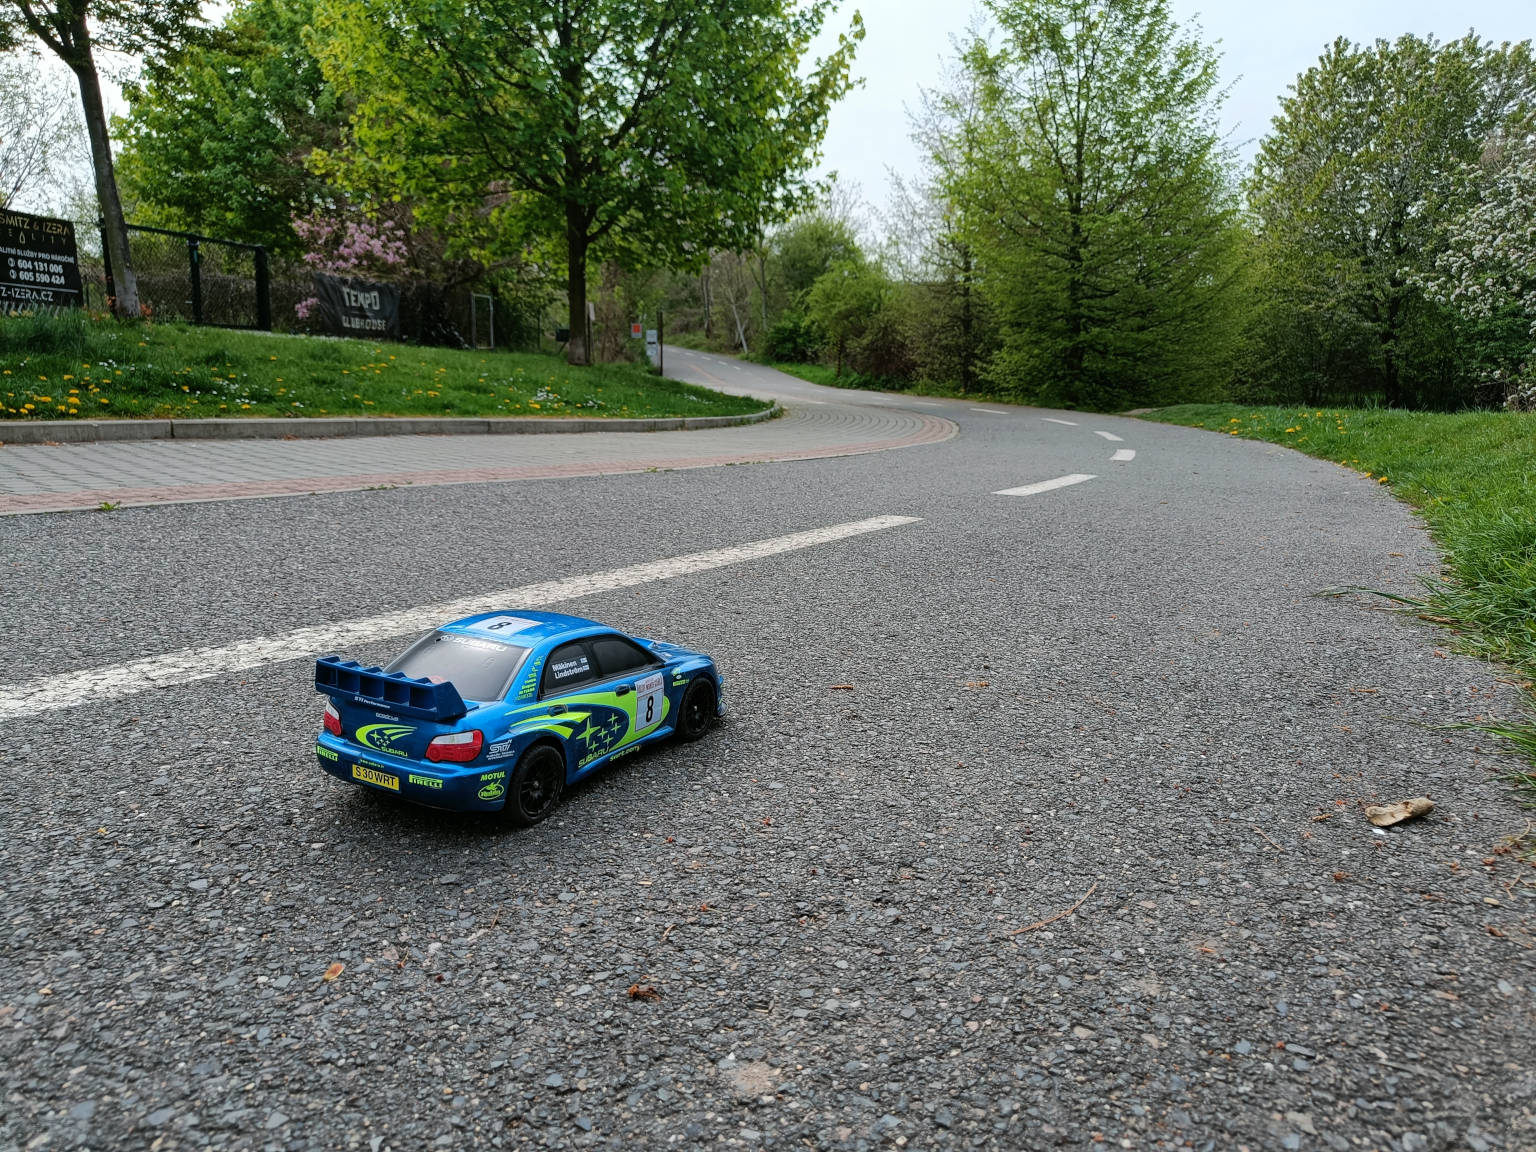
\includegraphics[width=0.8\linewidth]{images/placeholder}
\label{tab:BLDC_spec}
\end{table}

\begin{table}[t]
\caption{*PLACEHOLDER* ESC specifications} %TODO citace
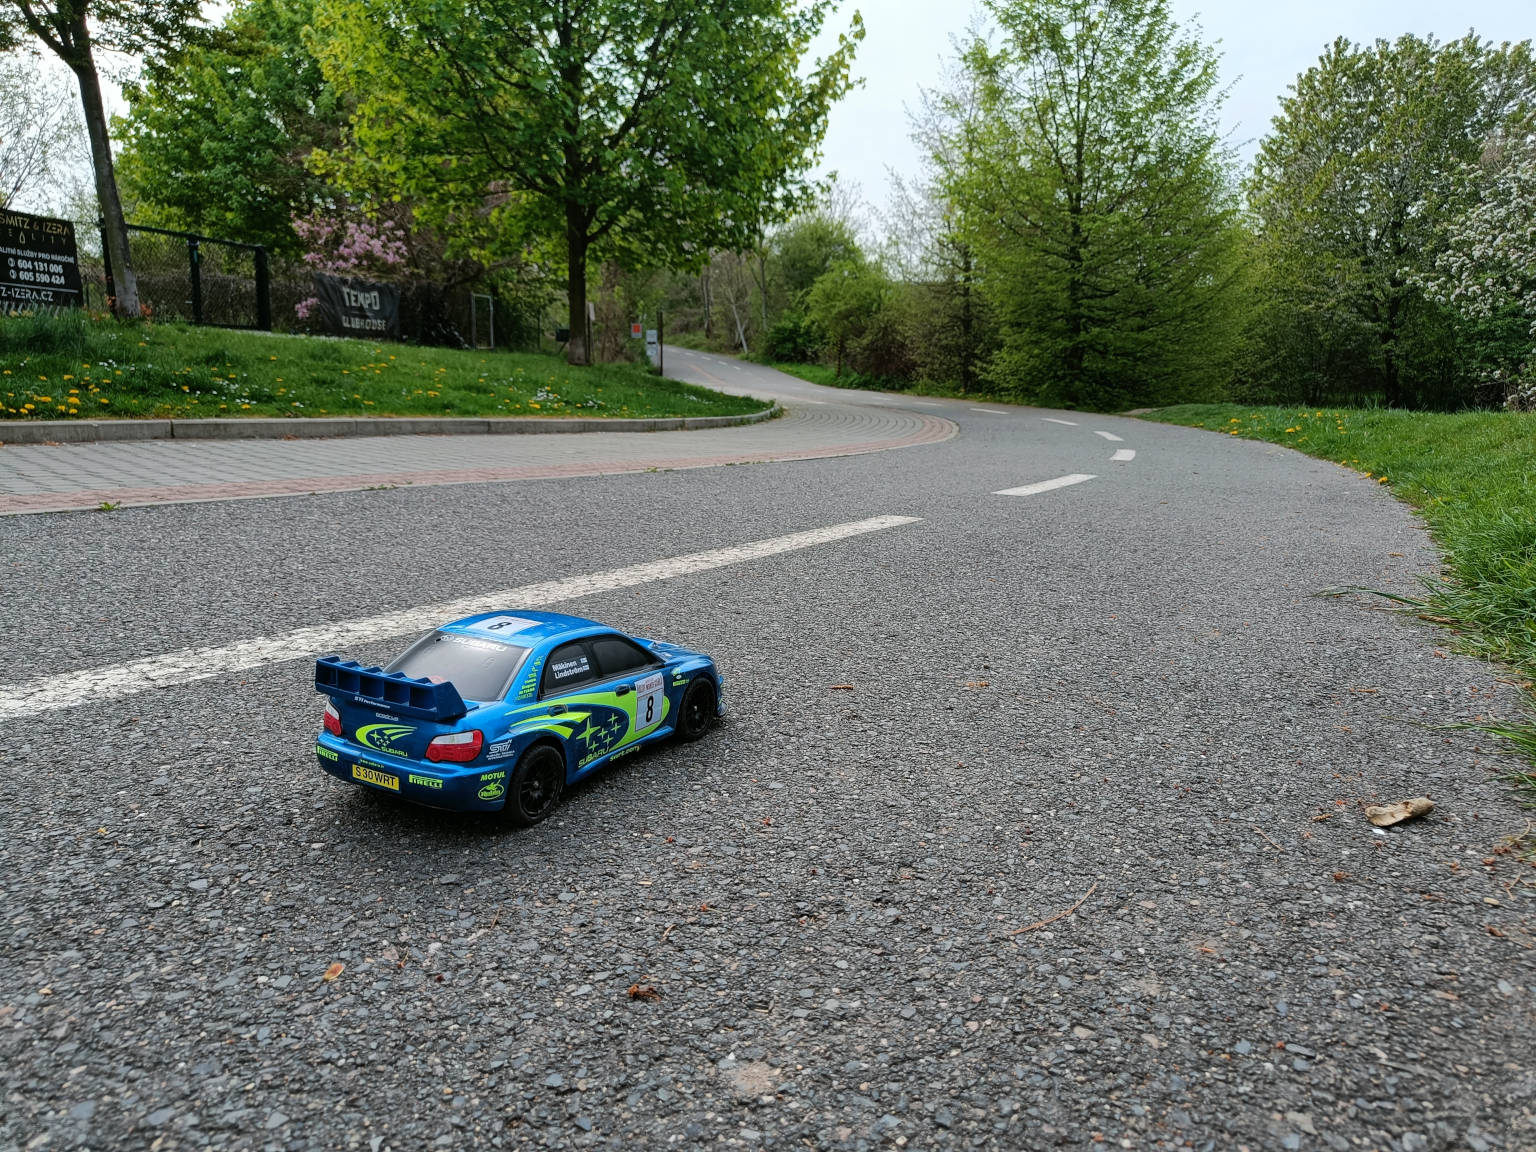
\includegraphics[width=0.8\linewidth]{images/placeholder}
\label{tab:ESC_spec}
\end{table}
